\subsection{Rademacher Complexity bound for linear function classes}
In the following section, we will explore a simple exercise for bounding the Rademacher Complexity for linear function classes. We will first look into the important theorems and lemmas. Then, we will tackle the problem at the end of this section.

\subsubsection{Problem Statement}
\label{sec:rc_bound_lin_func_problem}

\textbf{Problem} : Let $\F$ be a linear function class defined as followed:
\begin{align*}
    \F = \bigCurl{
        f:\R^d \to \R \Big| f(x) = wx, \|w\|_2 \le R
    }
\end{align*}

\noindent Our objective is to prove the following Rademacher Complexity bound:
\begin{align*}
    \RC_n(\F) \le \tilde O \biggRound{
        \frac{R}{\sqrt{n}}
    }
\end{align*}

\noindent Before solving the above problem, we have to get familiar with the definition of \textbf{covering number} and some related lemmas.


\subsubsection{Covering Number}
\begin{definition}[$\epsilon$-Cover]
    Let $Q$ be a set. A subset $\mathcal{C}\subset Q$ is called an \textbf{$\epsilon$-cover} of $Q$ with respect to a metric $\rho$ if:
    \begin{align*}
        \forall v \in Q, \exists v'\in \mathcal{C} : \rho(v, v') \le \epsilon
    \end{align*}

    \noindent Basically, $\mathcal{C}$ can be thought of as a collection of centers of \textbf{$\epsilon$-balls overlapping $Q$} (Figure \ref{fig:epsilon_cover}).
\end{definition}

\begin{figure}[ht]
    \centering
    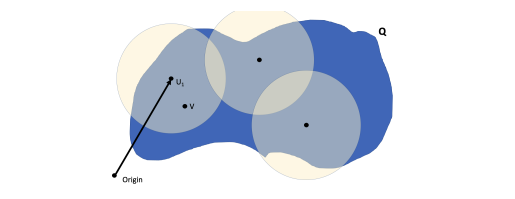
\includegraphics[width=\textwidth]{figures/epsilon_cover.png}
    \caption{Examples of $\epsilon$-balls. The centers of the balls would form an $\epsilon$-cover if they completely contain $Q$.}
    \label{fig:epsilon_cover}
\end{figure}

\begin{definition}[Covering Number of sets ($\mathcal{N}(Q, \epsilon, \rho$)]
    The \textbf{covering number} of a set $Q$ is defined as the size of the smallest $\epsilon$-cover needed to completely contain $Q$. In other words, it is the minimum number of $\epsilon$-balls needed to completely contain $Q$:
    \begin{align*}
        \mathcal{N}(Q, \epsilon, \rho) = \text{minimum size of $\epsilon$-cover of $Q$ w.r.t $\rho$}
    \end{align*}

    \noindent Visual illustration of covering number is included in figure \ref{fig:covering_number}.
\end{definition}

\begin{figure}[ht]
    \centering
    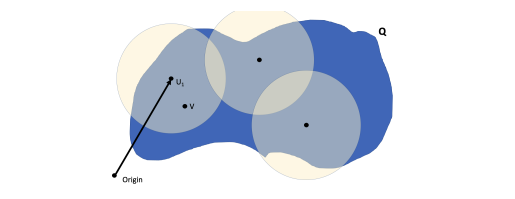
\includegraphics[width=\textwidth]{figures/covering_number.png}
    \caption{Example of covering number. For $\F$, the covering number is 5. For $\F'$, the covering number is 10.}
    \label{fig:covering_number}
\end{figure}


\begin{definition}[Covering number of function class ($\mathcal{N}(\F, \epsilon, \rho)$)]
    Let $\F$ be a function class. Define the restriction of $\F$ to the observations $\{x_1, \dots, x_n\}$ as:
    \begin{align*}
        \F_{x_1, \dots, x_n} = \bigCurl{
            (f(x_1), \dots, f(x_n)) : f \in \F
        }
    \end{align*}

    \noindent Then, we can define the \textbf{Covering Number} for $\F$ as followed:
    \begin{align*}
        \mathcal{N}(\F, \epsilon, \rho) = \sup_{x_1, \dots, x_n} \mathcal{N}(\F_{x_1, \dots, x_n}, \epsilon, \rho)
    \end{align*}

    \noindent We can call $\mathcal{N}(\F_{x_1, \dots, x_n}, \epsilon, \rho)$ the \textbf{Empirical Covering Number}.
\end{definition}

\subsubsection{Massart's Lemma}
\begin{theorem}{Massart's Lemma}{massart_lemma}
    Let $A\subseteq \R^n$ and $|A|<\infty$. Let $r=\sup_{u\in A}\|u\|_2$ ($\|.\|_2$ is the $l^2$ norm). Then,
    \begin{align*}
        \mathbb{E}_\sigma\biggSquare{
            \frac{1}{n} \sup_{u\in A}\sum_{i=1}^n \sigma_iu_i 
        } \le \frac{r\sqrt{2\ln|A|}}{n}
    \end{align*}

    \noindent Where $u = \begin{pmatrix} u_1 & \dots & u_n \end{pmatrix}^T$.
\end{theorem}

\begin{proof*}[Theorem \ref{thm:massart_lemma}]
    For all $t\ge0$, we have:
    \begin{align*}
        \exp\biggRound{
            t\E_\sigma\biggSquare{
                \sup_{u\in A} \sum_{i=1}^n \sigma_i u_i
            }
        } &= \exp\biggRound{
            \E_\sigma\biggSquare{
                t\sup_{u\in A} \sum_{i=1}^n \sigma_i u_i
            }
        } \\
        &\le \E_\sigma \biggSquare{
            \exp\biggRound{
                t\sup_{u\in A} \sum_{i=1}^n \sigma_i u_i
            }
        } \ \ \ (\text{Jensen's Inequality}) \\
        &= \E_\sigma \biggSquare{
            \sup_{u\in A} \exp\biggRound{
                t\sum_{i=1}^n \sigma_i u_i
            }
        } \ \ \ (\text{Exponential is strictly increasing}) \\
        &\le \sum_{u \in A} \E_\sigma\biggSquare{
            \exp\biggRound{
                t\sum_{i=1}^n \sigma_i u_i
            }
        }
    \end{align*}

    \noindent Since all Rademacher variables $\sigma_i$ are independent, we have:
    \begin{align*}
        \exp\biggRound{
            t\E_\sigma\biggSquare{
                \sup_{u\in A} \sum_{i=1}^n \sigma_i u_i
            }
        } &\le \sum_{u \in A} \prod_{i=1}^n \mathbb{E}_{\sigma_i} \bigSquare{
            \exp(t\sigma_iu_i)
        } \\
        &= \sum_{u \in A} \prod_{i=1}^n M_{\sigma_i} (tu_i)
    \end{align*}

    \noindent We know that $\E[\sigma_i]=0$ for every $1\le i \le n$ and $-1\le \sigma_i \le 1$ with probability $1$. Hence, by Hoeffding's lemma \ref{lem:hoeffding_lemma}, we have:
    \begin{align*}
        \exp\biggRound{
            t\E_\sigma\biggSquare{
                \sup_{u\in A} \sum_{i=1}^n \sigma_i u_i
            }
        } &\le \sum_{u \in A} \prod_{i=1}^n M_{\sigma_i} (tu_i) \\
        &\le \sum_{u \in A} \prod_{i=1}^n \exp\biggRound{
            \frac{4t^2u_i^2}{8}
        } = \sum_{u \in A} \prod_{i=1}^n \exp\biggRound{
            \frac{t^2u_i^2}{2}
        } \\
        &=  \sum_{u \in A} \exp\biggRound{
            \frac{t^2}{2}\sum_{i=1}^n u_i^2
        } \\
        &=  \sum_{u \in A} \exp\biggRound{
            \frac{t^2\|u\|_2^2}{2}
        } \\
        &\le  \sum_{u \in A} \exp\biggRound{
            \frac{t^2r^2}{2}
        } = |A|\exp\biggRound{
            \frac{t^2r^2}{2}
        }
    \end{align*}

    \noindent Taking the log from both sides, we have:
    \begin{align*}
        t\E_\sigma\biggSquare{
            \sup_{u\in A} \sum_{i=1}^n \sigma_i u_i
        } &\le \log|A| + \frac{t^2r^2}{2} \\
        \implies \E_\sigma\biggSquare{
            \sup_{u\in A} \sum_{i=1}^n \sigma_i u_i
        } &\le \inf_{t>0} \biggRound{
            \frac{\log|A|}{t} + \frac{tr^2}{2}
        }
    \end{align*}

    \noindent Setting the right hand side's derivative with respect to $t\ge0$ to $0$, we find that $t = r^{-1}\sqrt{2\log|A|}$. Plugging this value into the above bound, we have:
    \begin{align*}
        \E_\sigma\biggSquare{
            \sup_{u\in A} \sum_{i=1}^n \sigma_i u_i
        } &\le r\sqrt{2\log|A|}
    \end{align*}
\end{proof*}

\begin{corollary}{Massart's lemma bound on $\ERC_S(\F)$}{massart_lemma_bound_on_rc}
    Let $\F$ be a function class and let $Q$ be its output space. Given a dataset $S=\{x_1, \dots, x_n\}$, define the following norm for every $f\in\F$:
    \begin{align*}
        \|f\|_2 = \sqrt{
            \frac{1}{n}\sum_{i=1}^n f(x_1)^2
        }
    \end{align*}

    \noindent Then, we have the following bound on the Empirical Rademacher Complexity:
    \begin{align*}
        \ERC_S(\F) \le \sup_{f\in\F}\|f\|_2 \sqrt{
            \frac{2\log|\F|}{n}
        }
    \end{align*}
\end{corollary}

\begin{proof*}[Corollary \ref{coro:massart_lemma_bound_on_rc}]
    Let $r=\sup_{q\in Q} \|q\|_2$ where the norm applied on the output space is the $l^2$ norm (without the scaling factor $\frac{1}{\sqrt n}$). We have:
    \begin{align*}
        \sup_{f\in\F}\|f\|_2 
            &= \sup_{f\in\F} \sqrt{
                \frac{1}{n} \sum_{i=1}^n f(x_i)^2
            } \\
            &= \frac{1}{\sqrt{n}} \sup_{q \in Q}\sqrt{
                \sum_{i=1}^n q_i^2
            } \\
            &= \frac{r}{\sqrt n} \\
        \implies 
        r &= \sqrt{n}\sup_{f\in\F}\|f\|_2 
    \end{align*} 

    \noindent We have:
    \begin{align*}
        \ERC_S(\F) &= \mathbb{E}_\sigma \biggSquare{
            \sup_{f\in\F}\frac{1}{n}\sum_{i=1}^n\sigma_i f(x_i)
        } \\
        &= \mathbb{E}_\sigma \biggSquare{
            \sup_{q\in Q}\frac{1}{n}\sum_{i=1}^n\sigma_i q_i
        } \\
        &\le \frac{r\sqrt{2\log|Q|}}{n} \ \ \ (\text{Massart's lemma \ref{thm:massart_lemma}}) \\
        &= \sup_{f\in\F}\|f\|_2 \frac{\sqrt{2n\log|Q|}}{n} \\
        &= \sup_{f\in\F}\|f\|_2 \sqrt{\frac{2\log|\F|}{n}}
    \end{align*}
\end{proof*}


\subsubsection{Dudley's Theorem}
\begin{theorem}{Dudley's Theorem}{dudley_theorem}
    If $\F$ is a function class from $\mathcal{Z}\to\R$ (where $\mathcal{Z}$ is a vector space and the norm of $f\in\F$ is not necessarily bounded), then:
    \begin{align*}
        \ERC_S(\F) \le 12\int_0^{\sup_{f\in\F}\|f\|_2} \sqrt{
            \frac{\log \mathcal{N}(\F, \epsilon, \|.\|_2)}{n}
        }d\epsilon
    \end{align*}

    \noindent Where for any $f\in\F$, given a sample $x_1, \dots, x_n$, we define the $\|.\|_2$ norm as followed:
    \begin{align*}
        \|f\|_2 = \sqrt{
            \frac{1}{n}\sum_{i=1}^n f(x_i)^2
        }
    \end{align*}
\end{theorem}
\begin{proof*}[Theorem \ref{thm:dudley_theorem}]
    The main idea of the proof is via chaining. Define the following sequence $\{\epsilon_j\}_{j=0}^n$:
    \begin{align*}
        \begin{cases}
            \epsilon_0 &= \sup_{f\in\F} \|f\|_2
            \\ 
            \epsilon_j &= 2^{-j}\epsilon_0
        \end{cases}
    \end{align*}

    \noindent Next, we define the sequence of $\epsilon$-covers $\mathcal{N}_{\epsilon_j}$ corresponding to each $\epsilon_j$. By definition, we have:
    \begin{align*}
        \forall f\in\F, \exists g_j \in \mathcal{N}_{\epsilon_j} : \|f-g_j\|_2 \le \epsilon_j
    \end{align*}

    \noindent We can write any $f\in\F$ as the following telescoping sum:
    \begin{align*}
        f = f - g_n + \sum_{j=1}^n \bigRound{g_j - g_{j-1}}
    \end{align*}

    \noindent Now, define the Empirical Rademacher Complexity as followed:
    \begin{align*}
        \ERC_S(\F) = \E_\sigma\biggSquare{
            \sup_{f\in\F} \frac{1}{n} \sum_{i=1}^n \sigma_i f(x_i) 
        } = \E_\sigma\biggSquare{
            \sup_{f\in\F} \big< \sigma, f \big> \Bigg| x_1, \dots, x_n
        }
    \end{align*}

    \noindent We have:
    \begin{align*}
        \ERC_S(\F) &= \E_\sigma\biggSquare{
            \sup_{f\in\F} \big< \sigma, f \big> \Bigg| x_1, \dots, x_n
        }\\
        &= \E_\sigma\biggSquare{
            \sup_{f\in\F} \Big< \sigma, f - g_n + \sum_{j=1}^n \bigRound{g_j - g_{j-1}} \Big> \Bigg| x_1, \dots, x_n
        } \\
        &\le \E_\sigma\biggSquare{
            \sup_{f\in\F} \big< \sigma, f-g_n\big> + \sup_{f\in\F} \sum_{j=1}^n \big<\sigma, g_j - g_{j-1}\big> \Bigg| x_1, \dots, x_n
        } \ \ \ (\sup\Sigma \le \Sigma\sup) \\
        &\le \|\sigma\|_2\cdot\|f-g_n \|_2 + \E_\sigma\biggSquare{
            \sup_{f\in\F} \sum_{j=1}^n \big<\sigma, g_j - g_{j-1}\big> \Bigg| x_1, \dots, x_n
        } \ \ \ (\text{Cauchy-Schwarz}) \\
        &\le \epsilon_n + \E_\sigma\biggSquare{
            \sup_{f\in\F} \sum_{j=1}^n \big<\sigma, g_j - g_{j-1}\big> \Bigg| x_1, \dots, x_n
        } \\
        &\le \epsilon_n + \sum_{j=1}^n \E_\sigma\biggSquare{
            \sup_{f\in\F} \big<\sigma, g_j - g_{j-1}\big> \Bigg| x_1, \dots, x_n
        }
    \end{align*}

    \noindent From here, note that:
    \begin{align*}
        \|g_j - g_{j-1}\|_2 \le \|g_j - f\|_2 + \|g_{j-1}-f\|_2 \le \epsilon_j + \epsilon_{j-1} = 3\epsilon_j
    \end{align*}

    \noindent Also, define the following classes of functions:
    \begin{align*}
        \Hf_j = \bigCurl{
            g_j - g_{j-1}\Big| 
            g_j \in \mathcal{N}_{\epsilon_j},
            g_{j-1} \in \mathcal{N}_{\epsilon_{j-1}}
        }
    \end{align*}

    \noindent Continuing the above, we have:
    \begin{align*}
        \ERC_S(\F) &\le \epsilon_n + \sum_{j=1}^n \E_\sigma\biggSquare{
            \sup_{h\in\Hf_j} \big<\sigma, h \big> \Bigg| x_1, \dots, x_n
        } \\
        &= \epsilon_n + \sum_{j=1}^n \ERC_S(\Hf_j) \\
        &\le  \epsilon_n + \sum_{j=1}^n \sup_{h\in \Hf_j} \|h\|_2 \cdot \sqrt{
            \frac{2\log|\Hf_j|}{n}
        } \ \ \ (\text{Massart's lemma}) \\
        &\le \epsilon_n + \sum_{j=1}^n 6(\epsilon_j - \epsilon_{j-1}) \cdot \sqrt{
            \frac{2\log|\Hf_j|}{n}
        } \ \ \ \Big(\sup_{h\in \Hf_j} \|h\|_2 \le 3\epsilon_j \le 6(\epsilon_j - \epsilon_{j+1})\Big)
    \end{align*}

    \noindent Now we have:
    \begin{align*}
        |\Hf_j| \le |\mathcal{N}_{\epsilon_j}| \cdot |\mathcal{N}_{\epsilon_{j-1}}| \le |\mathcal{N}_{\epsilon_j}|^2
    \end{align*}

    \noindent Hence, we have:
    \begin{align*}
        \ERC_S(\F) &\le \epsilon_n + 6\sum_{j=1}^n (\epsilon_j - \epsilon_{j-1}) \cdot \sqrt{
            \frac{2\log|\mathcal{N}_{\epsilon_j}|^2}{n}
        } \\
        &= \epsilon_n + 12\sum_{j=1}^n (\epsilon_j - \epsilon_{j-1}) \cdot \sqrt{
            \frac{\log|\mathcal{N}_{\epsilon_j}|}{n}
        } \\
        &\le \epsilon_n + 12\sum_{j=1}^n \int_{\epsilon_{j+1}}^{\epsilon_j} \sqrt{
            \frac{\log|\mathcal{N}_{\epsilon_j}|}{n}
        }dt \\
        &\le \epsilon_n + 12\sum_{j=1}^n \int_{\epsilon_{j+1}}^{\epsilon_j} \sqrt{
            \frac{\log|\mathcal{N}_t|}{n}
        }dt \\
        &\le  \epsilon_n + 12 \int_{\epsilon_{n+1}}^{\epsilon_0} \sqrt{
            \frac{\log|\mathcal{N}_t|}{n}
        }dt
    \end{align*}

    \noindent Now take $n\to\infty$, we notice that $\epsilon_n\to0$ and the above inequality holds for every $\epsilon$-cover for $0<\epsilon<\epsilon_0=\sup_{f\in\F}\|f\|_2$. Therefore,
    \begin{align*}
        \ERC_S(\F) &\le 12 \int_{0}^{\sup_{f\in\F}\|f\|_2} \sqrt{
            \frac{\log\mathcal{N}(\F, \epsilon, \|.\|_2)}{n}
        }d\epsilon
    \end{align*}
\end{proof*}

\noindent\newline\textbf{Remark} : Using theorem \ref{thm:dudley_theorem}, we can translate the covering number to the Empirical Rademacher Complexity given that the covering number has some special formulation and the function class $\F$ is bounded in $[-1, 1]$. For example:
\begin{itemize}
    \item ${\bf (i)} \ \mathcal{N}(\F, \epsilon, \|.\|_2) \approx (1/\epsilon)^R$.

    \noindent Then we have $\log\mathcal{N}(\F, \epsilon, \|.\|_2) \approx R\log(1/\epsilon)$. Therefore,
    \begin{align*}
        \int_0^1 \sqrt{
            \frac{\log \mathcal{N}(\F, \epsilon, \|.\|_2)}{n}
        }d\epsilon = \int_0^1\sqrt{
            \frac{R\log(1/\epsilon)}{n}
        }d\epsilon \approx \sqrt{\frac{R}{n}}
    \end{align*}

    \item ${\bf (ii)} \ \mathcal{N}(\F, \epsilon, \|.\|_2) \approx a^{R/\epsilon}$.

    \noindent Then we have $\log\mathcal{N}(\F, \epsilon, \|.\|_2) \approx \frac{R}{\epsilon}\log a$. Therefore,
    \begin{align*}
        \int_0^1 \sqrt{
            \frac{\log \mathcal{N}(\F, \epsilon, \|.\|_2)}{n}
        }d\epsilon &\approx \int_0^1\sqrt{
            \frac{R}{n\epsilon}\log a 
        }d\epsilon \\
        &= \sqrt{
            \frac{R}{n}\log a 
        }\int_0^1 \sqrt{\frac{1}{\epsilon}}d\epsilon \\
        &= \tilde O\biggRound{ \sqrt{\frac{R}{n}} }
    \end{align*}

    \item ${\bf (iii)} \ \mathcal{N}(\F, \epsilon, \|.\|^2) \approx a^{R/\epsilon^2}$.
    
    \noindent Then, we have $\log \mathcal{N}(\F, \epsilon, \|.\|^2)\approx \frac{R}{\epsilon^2}\log a$. Therefore,
    \begin{align*}
        \int_0^1 \sqrt{
            \frac{\log \mathcal{N}(\F, \epsilon, \|.\|^2)}{n}
        }d\epsilon \approx \sqrt{
            \frac{R}{n}\log a 
        }\int_0^1 \frac{1}{\epsilon}d\epsilon = \infty
    \end{align*}
\end{itemize}


\subsubsection{Bound on covering number of linear function class}
\begin{theorem}{Maurey's Sparsification Lemma}{maurey_sparsification_elmma}
    In a Hilbert space $\Hf$ equiped with a norm $\|.\|$, let $f\in\Hf$ where $f=\sum_{j=1}^d w_jg_j, \ \ g_j\in\Hf$ such that $\|g_j\| \le b, w_j \ge 0$ and $\alpha=\sum_{j=1}^d w_j \le 1$. Then, for any $n\ge1$, there exists non-negative integers $k_1, \dots, k_d\ge0$ such that $\sum_{j=1}^d k_j \le n$ and:
    \begin{align*}
        \Bigg\|
            f - \sum_{j=1}^d \frac{k_j}{n} g_j 
        \Bigg\|^2
        \le \frac{\alpha b^2 - \|f\|^2}{n}
    \end{align*}
\end{theorem}

\noindent \textbf{Remark} : The intuition of theorem \ref{thm:maurey_sparsification_elmma} is that if we have a function from a Hilbert space which can be written as linear combination of bounded functions. Then, we can estimate the coefficients $w_j$ using integer solutions $k_j$. The higher $n$ gets, the more accurately we can estimate the coefficients.

\begin{proof*}[Theorem \ref{thm:maurey_sparsification_elmma}]
    The proof of this theorem is too technical for this note. However, a rigorous proof is provided in the following paper \cite{article:bartlett} (Lemma A.6).
\end{proof*}

\begin{lemma}{Bound on $\mathcal{N}(\F, \epsilon, \|.\|_2)$ for linear functions}{covering_num_bound_lin_func}
    Let $\F$ be a linear function class defined as followed:
    \begin{align*}
        \F = \bigCurl{
            f:\R^d\to\R \Big| f(x) = wx, \|w\|_q \le a, \|x\|_p \le b
        }
    \end{align*}

    \noindent Where $p, q$ are Holder conjugates and $2\le p\le \infty$. Then, we have:
    \begin{align*}
        \log\mathcal{N}(\F, \epsilon, \|.\|_2) \le \Bigg\lceil \frac{a^2b^2}{\epsilon^2} \Bigg\rceil \log(2d+1)
    \end{align*}

    \noindent The proof of this lemma is discussed in Theorem 3 in \cite{article:tong_zhang}.
\end{lemma}
\begin{proof*}[Lemma \ref{lem:covering_num_bound_lin_func}]
    For $f\in\F$, we can write:
    \begin{align*}
        f(x) &= \sum_{j=1}^d x_j \cdot w_j \\
        \|x\|_p &= \biggRound{
            \sum_{j=1}^d |x_j|^p
        }^{1/p} \le b \\
        \|w\|_q &= \biggRound{
            \sum_{j=1}^d |w_j|^q
        }^{1/q} \le a
    \end{align*}

    \noindent We define the following:
    \begin{align*}
        g_j(x) &= \frac{n^{1/p}ab}{|x_j|}x_j, \ \ w_j' = \frac{|x_j|}{n^{1/p}ab}w_j, \ \ (n\ge1)
    \end{align*}

    \noindent By Holder's inequality, we can check that:
    \begin{align*}
        \sum_{j=1}^d |w_j'| 
            &= \sum_{j=1}^d \frac{|x_j|}{n^{1/p}ab} |w_j| \\
            &\le \frac{1}{n^{1/p}ab}\biggRound{
                \sum_{j=1}^d |x_j|^p
            }^{1/p}\biggRound{
                \sum_{j=1}^d |w_j|^q 
            }^{1/q} \\
            &= \frac{\|x\|_p \|w\|_q}{n^{1/p}ab} \\
            &\le \frac{1}{n^{1/p}} \\
            &\le 1
    \end{align*}

    \noindent By the definition of $g_j$, we know that:
    \begin{align*}
        \forall x \in \R^d : g_j(x) \le n^{1/p}ab \implies \|g_j\|_2 \le n^{1/2}ab
    \end{align*}

    \noindent Furthermore, for all $f\in\F$, we can write:
    \begin{align*}
        f(x) = \sum_{j=1}^d w_j x_j \implies f := \sum_{j=1}^{d}|w_j'|\cdot[sgn(w_j')g_j]
    \end{align*}

    \noindent Hence, if we choose $\lceil (ab/\epsilon)^2 \rceil \ge K \ge (ab/\epsilon)^2$, by theorem \ref{thm:maurey_sparsification_elmma}, we can always find integers $k_1, \dots, k_d$ such that $\sum_{j=1}^{d}|k_j| \le K$ and:
    \begin{align*}
        \Bigg\| 
            f - \sum_{j=1}^{d} \frac{k_j}{K}g_j
        \Bigg\|_2^2 
            &\le \frac{na^2b^2\sum_{j=1}^{d}|w_j'| - \|f\|_2^2}{K} \\
            &\le \frac{na^2b^2 - \|f\|_2^2}{K} \\
            &\le \frac{na^2b^2}{K} \\
            &\le n\epsilon^2
    \end{align*}

    \noindent \textbf{Remark} : Note that the above norm refers to the standard $l^2$ norm. However, when we switch to the norm used in covering number and Rademacher Complexity (with the scaling factor $\frac{1}{\sqrt n}$), the $n$ on the right-hand-side vanishes.

    \noindent\newline From the above, the covering number of $\F$ will not exceed the number of integer solutions for $\sum_{j=1}^{d}|k_j| \le K$, which is $(2d+1)^K$. Hence, we have:
    \begin{align*}
        \log\mathcal{N}(\F, \epsilon, \|.\|_2) &\le K\log(2d+1) \\
        &\le \Bigg\lceil \frac{a^2b^2}{\epsilon^2} \Bigg\rceil \log(2d+1)
    \end{align*}
\end{proof*}


\subsubsection{Rademacher Complexity bound for linear functions class}
In this section, we finally solve the problem stated in section \ref{sec:rc_bound_lin_func_problem}. First, consider the following lemma, then prove the proposition \ref{prop:rc_bound_for_lin_func}:

\begin{theorem}{Dudley's Entropy Integral bound}{dudley_entropy_integral}
    Let $\F$ be a real-valued function class and assume that ${\bf 0}\in\F$, $S=\{x_1, \dots, x_n\}$ is a dataset. Then,
    \begin{align*}
        \ERC_S(\F) \le \inf_{\alpha>0} \biggRound{
            4\alpha + 12\int_\alpha^{\sup_{f\in\F}\|f\|_2} \sqrt{
                \frac{\log\mathcal{N}(\F, \epsilon,\|.\|_2)}{n}
            }d\epsilon
        }
    \end{align*}

    \noindent Where we define the $\|.\|_2$ norm as followed:
    \begin{align*}
        \|f\|_2 = \sqrt{
            \frac{1}{n}\sum_{i=1}^n f(x_i)^2
        }, \ f\in\F
    \end{align*}
\end{theorem}
\begin{proof*}[Theorem \ref{thm:dudley_entropy_integral}]
    This proof extend the proof for the more general Dudley's theorem \ref{thm:dudley_theorem}. From the proof, we have:
    \begin{align*}
        \ERC_S(\F) &\le \epsilon_n + 12 \int_{\epsilon_{n+1}}^{\epsilon_0} \sqrt{
            \frac{\log\mathcal{N}(\F, \epsilon, \|.\|_2)}{n}
        }dt
    \end{align*}

    \noindent Where $\epsilon_0=\sup_{f\in\F}\|f\|_2$ and for every $j\ge1$ we have $\epsilon_j = 2^{-j}\epsilon_0$. $\mathcal{N}(\F, \epsilon, \|.\|_2)$ is the size of the minimum $\epsilon$-cover.

    \noindent\newline Let $\alpha\ge0$, pick the sample size $n$ such that:
    \begin{align*}
        n = \sup_{j\ge1} \bigCurl{j : \epsilon_j \ge 2\alpha}
    \end{align*}

    \noindent Hence, for any choice of sample size of at least $n+1$, we have:
    \begin{align*}
        \epsilon_{n+1} \le 2\alpha \implies \epsilon_n = 2\epsilon_{n+1} \le 4\alpha
    \end{align*}

    \noindent We also have:
    \begin{align*}
        \epsilon_{n+1} = \frac{\epsilon_n}{2} \ge \frac{2\alpha}{2} = \alpha
    \end{align*}

    \noindent Therefore, we have:
    \begin{align*}
        \ERC_S(\F) &\le \epsilon_n + 12 \int_{\epsilon_{n+1}}^{\epsilon_0} \sqrt{
            \frac{\log\mathcal{N}(\F, \epsilon, \|.\|_2)}{n}
        }dt \\
        &\le 4\alpha + 12 \int_{\epsilon_{n+1}}^{\epsilon_0} \sqrt{
            \frac{\log\mathcal{N}(\F, \epsilon, \|.\|_2)}{n}
        }dt \ \ \ (\epsilon_n \le 4\alpha) \\
        &\le 4\alpha + 12 \int_{\alpha}^{\epsilon_0} \sqrt{
            \frac{\log\mathcal{N}(\F, \epsilon, \|.\|_2)}{n}
        }dt \ \ \ (\epsilon_{n+1} \ge \alpha) \\
        &=  4\alpha + 12 \int_{\alpha}^{\sup_{f\in\F}\|f\|_2} \sqrt{
            \frac{\log\mathcal{N}(\F, \epsilon, \|.\|_2)}{n}
        }dt 
    \end{align*}

    \noindent Since the left-hand-side does not depend on $\alpha$, we can take the infimum over $\alpha>0$ to obtain the tightest bound:
    \begin{align*}
        \ERC_S(\F) &\le \inf_{\alpha>0}\biggRound{
            4\alpha + 12 \int_{\alpha}^{\sup_{f\in\F}\|f\|_2} \sqrt{
                \frac{\log\mathcal{N}(\F, \epsilon, \|.\|_2)}{n}
            }dt 
        }
    \end{align*}
\end{proof*}

\begin{proposition}{$\RC_n(\F)$ bound for linear function class (covering number)}{rc_bound_for_lin_func}
    Given the following function class $\F$ whose range is bounded within $[-1, 1]$:
    \begin{align*}
        \F = \bigCurl{
            f:\R^d\to\R \Big| f(x) = wx, \|w\|_2 \le a, \|x\|_2 \le b
        }
    \end{align*}

    \noindent Then, we can obtain the following bound for the Rademacher Complexity using Covering number:
    \begin{align*}
        \RC_n(\F) \le \tilde O \biggRound{\frac{R}{\sqrt{n}}}, \ \ R = ab
    \end{align*}
\end{proposition}
\begin{proof*}[Proposition \ref{prop:rc_bound_for_lin_func}]
    \noindent From lemma \ref{lem:covering_num_bound_lin_func}, we have the following bound on the covering number of $\F$:
    \begin{align*}
        \log\mathcal{N}(\F, \epsilon, \|.\|_2) \le \Bigg\lceil \frac{R^2}{\epsilon^2} \Bigg\rceil \log(2d+1) < 2\frac{R^2}{\epsilon^2}\log(2d+1) = \frac{R^2}{\epsilon^2}\log(4d^2 + 4d + 1)
    \end{align*}

    \noindent The second inequality holds under the assumption that $R^2 > \epsilon^2$. Let $D = 4d^2 + 4d + 1$, we have:
    \begin{align*}
        \log\mathcal{N}(\F, \epsilon, \|.\|_2) < \frac{R^2}{\epsilon^2} \log D
    \end{align*}

    \noindent Since $\F$ is bounded in the $[-1, 1]$ range, we have that $\sup_{f\in\F}\|f\|_2 \le 1$. Hence, we have:
    \begin{align*}
        \int_\alpha^{\sup_{f\in\F}\|f\|_2} \sqrt{\log\mathcal{N}(\F, \epsilon, \|.\|_2)} d\epsilon
            &\le \int_\alpha^1 \sqrt{\log\mathcal{N}(\F, \epsilon, \|.\|_2)} d\epsilon \\
            &< R\sqrt{\log D}\int_\alpha^1 \frac{1}{\epsilon}d\epsilon \\
            &= R\sqrt{\log D}\bigRound{ - \log\alpha }
    \end{align*}

    \noindent Using theorem \ref{thm:dudley_entropy_integral}, we have:
    \begin{align*}
        \ERC_S(\F) 
            &\le \inf_{\alpha>0}\biggRound{
                4\alpha + \frac{12}{\sqrt n} \int_\alpha^{\sup_{f\in\F}\|f\|_2} \sqrt{\log\mathcal{N}(\F, \epsilon, \|.\|_2)} d\epsilon
            } \\
            &< \inf_{\alpha>0}\biggRound{
                4\alpha + \frac{12}{\sqrt n} R\sqrt{\log D} \bigRound{ - \log\alpha }
            }
    \end{align*}

    \noindent Letting $\alpha=\frac{3R}{\sqrt n}$, we have:
    \begin{align*}
        \ERC_S(\F) &< \frac{12R}{\sqrt n} + \frac{12R}{\sqrt n}\sqrt{\log D} \biggRound{ - \log\frac{3R}{\sqrt n} } \\
        &= \frac{12R}{\sqrt n} \biggSquare{
            1 - \sqrt{\log D}\log\frac{3R}{\sqrt{n}}
        } \\
        &= \tilde O\biggRound{ \frac{R}{\sqrt n} }
    \end{align*}

    \noindent Since the right-hand-side does not depend on the sample $S$, we can just take expectation over the samples for both sides and we have:
    \begin{align*}
        \RC_n(\F) < \tilde O\biggRound{ \frac{R}{\sqrt n} }
    \end{align*}

    \noindent \textbf{Remark} : In fact, we do not have to specify the bound range $[-1, 1]$ of $\F$ and make the above result more general:
    \begin{align*}
        \ERC_S(\F) &< \frac{12R}{\sqrt n}\biggSquare{
            1 + \log\sup_{f\in\F}\|f\|_2 - \sqrt{\log D}\log\frac{3R}{\sqrt{n}}
        } = \tilde O\biggRound{ \frac{R}{\sqrt n} }
    \end{align*}
\end{proof*}


\begin{proposition}{$\RC_n(\F)$ bound for linear function class (no covering number)}{rc_bound_for_lin_func_wo_covering_number}
    The following proposition presents an upper bound for the Rademacher Complexity without dependence on the dimensionality $d$. Let $\F$ be a function class (not necessarily linear) and $Q$ is its output space such that:
    \begin{align*}
        R = \sup_{q\in Q} \|q\|_2
    \end{align*}

    \noindent Then, we have the following bound on the Rademacher Complexity:
    \begin{align*}
        R_n(\F) \le \frac{R}{\sqrt n}
    \end{align*}
\end{proposition}

\begin{proof*}[Proposition \ref{prop:rc_bound_for_lin_func_wo_covering_number}]
    Let $S$ be samples with $n$ elements, we have:
    \begin{align*}
        \RC_n(\F) 
            &= \frac{1}{n}\E_S\E_\sigma \biggSquare{
                \sup_{q\in Q} \big< \sigma, q \big>
            } \\
            &\le \frac{1}{n} \E_S\E_\sigma \biggSquare{
                \sup_{q\in Q} \|\sigma\|_2 \cdot \|q\|_2
            } \ \ \ (\text{Cauchy-Schwarz}) \\
            &= \frac{1}{n} \E_S\E_\sigma \biggSquare{
                \|\sigma\|_2 \cdot \sup_{q\in Q} \|q\|_2
            } \\
            &= \frac{R}{n} \E_S\E_\sigma \bigSquare{\|\sigma\|_2} \\
            &= \frac{R}{n} \E_\sigma \bigSquare{\|\sigma\|_2} \\
            &= \frac{R}{n} \E_\sigma \biggSquare{
                \sqrt{
                    \sum_{i=1}^n \sigma_i^2
                }
            } \\
            &\le \frac{R}{n}\sqrt{
                \sum_{i=1}^n \E_\sigma [\sigma_i^2]
            } \ \ \ (\text{Jenen's Inequality}) \\
            &= \frac{R}{\sqrt n}
    \end{align*}
\end{proof*}

